\mySection{Experimental Results}
We want to find out how many photos must be collected from each individual in order to have PyRollCall reach its best performance.
The results indicate that PyRollCall can achieve approximately \textbf{70\% to 85\%} of correct rate for facial recognition at its best
if \textbf{25 to 30} photos are collected in advance from each individual.
The raw data of our experiments is presented in table~\ref{tab:exp-result-tab},
and we also visualize the data with a line chart, as shown in figure~\ref{fig:exp-result-chart}.
\vspace{0.3cm}

\begin{table}[!htb]
\centering
\caption{Correct rate for PyRollCall's facial recognition feature.} 
\begin{tabular}{@{}lcccccc@{}}
\toprule[2pt]
& \multicolumn{6}{c}{Number of embeddings pre-computed per person}                                                                                                               \\ \addlinespace[0.5em]
              & 5                          & 10                         & 15                         & 20                         & 25                         & 30                         \\ \midrule \addlinespace[0.5em]
Testing Set 1 & 8/20                       & 10/20                      & 15/20                      & 17/20                      & 17/20                      & 17/20                      \\
              & \multicolumn{1}{c}{(40\%)} & \multicolumn{1}{c}{(50\%)} & \multicolumn{1}{c}{(75\%)} & \multicolumn{1}{c}{(85\%)} & \multicolumn{1}{c}{(85\%)} & \multicolumn{1}{c}{(85\%)} \\ \addlinespace[0.5em] \midrule \addlinespace[0.5em]
Testing Set 2 & 8/20                       & 10/20                      & 12/20                      & 13/20                      & 14/20                      & 14/20                      \\
              & \multicolumn{1}{c}{(40\%)} & \multicolumn{1}{c}{(50\%)} & \multicolumn{1}{c}{(60\%)} & \multicolumn{1}{c}{(65\%)} & \multicolumn{1}{c}{(70\%)} & \multicolumn{1}{c}{(70\%)} \\ \addlinespace[0.5em] \midrule \addlinespace[0.5em]
Testing Set 3 & 9/20                       & 13/20                      & 14/20                      & 15/20                      & 15/20                      & 15/20                      \\
              & \multicolumn{1}{c}{(45\%)} & \multicolumn{1}{c}{(65\%)} & \multicolumn{1}{c}{(70\%)} & \multicolumn{1}{c}{(75\%)} & \multicolumn{1}{c}{(75\%)} & \multicolumn{1}{c}{(75\%)} \\ \addlinespace[0.5em]
\bottomrule[2pt]
\end{tabular}
\label{tab:exp-result-tab}
\end{table}
\vspace{0.2cm}

\begin{figure}[!htb]
  \centering
  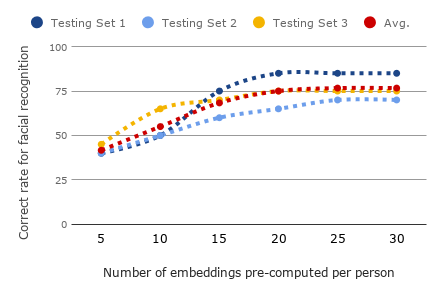
\includegraphics[width=0.85\linewidth]{figures/exp-result-chart.png}
  \caption{Visualization of the correct rate for PyRollCall's facial recognition feature.}
  \label{fig:exp-result-chart}
\end{figure}
\clearpage


With sufficient photos of students provided and their facial embeddings pre-computed,
the system will be able to detect and recognize faces correctly. Currently, as shown

to save time
in classes, teachers and students will have to spend equivilently extra amount of time
before classes on the tasks such as collecting photos and pre-computing facial embeddings.
This proves that there is a trade off between convenience and efficiency.
\vspace{0.2cm}

